\documentclass[12pt,a4paper]{article}
\usepackage[utf8]{inputenc}

% Bibliography management
\usepackage[
backend=biber
% citestyle=authoryear,
% style=alphabetic,
% sorting=ynt
]{biblatex}
\addbibresource{bibliography.bib}
% \usepackage[nottoc]{tocbibind}

% Code Listings
\usepackage{listings}
\usepackage{listings-golang} % import this package after listings
\usepackage{color}
\usepackage[dvipsnames]{xcolor}

% Images
% \usepackage{graphicx}
% \graphicspath{ {images/} }

% Diagrams
\usepackage{tikz}
\usetikzlibrary{shapes, arrows, arrows.meta, calc, fit}

\setlength{\abovecaptionskip}{5px}

\title{A compositional toolkit for the construction of concurrent Web servers}
\author{Michal Bock}
\date{}

\lstset{ % add your own preferences
    frame=single,
    basicstyle=\footnotesize,
    keywordstyle=\color{blue}\bfseries,
    numbers=none,
    showstringspaces=false, 
    stringstyle=\color{red},
    tabsize=4,
    language=Golang,
    belowskip=0px,
    emph={go},
    emphstyle={\color{blue}\bfseries},
    commentstyle={\color{ForestGreen}\textit},
    rulecolor=\color{black}
}

% Define block styles
\tikzstyle{listener} = [rectangle, draw, fill=gray!60, 
    text width=5em, text centered, minimum height=4em]
\tikzstyle{component} = [rectangle, draw, fill=white, 
    text width=5em, text centered, minimum height=4em]
\tikzstyle{writer} = [rectangle, draw, fill=gray!30, 
    text width=5em, text centered, minimum height=4em]
\tikzstyle{line} = [draw, -latex]
\tikzstyle{condition} = [draw, circle, fill=white, yshift=-0.3cm]

\tikzset{cross/.style n args={0}{
    minimum width=6mm,
    path picture={
        \draw[black, -] (path picture bounding box.south east) -- 
                     (path picture bounding box.north west);
        \draw[black, -] (path picture bounding box.south west) --
                     (path picture bounding box.north east);
        }
    }
}


\usepackage[parfill]{parskip}
\usepackage[labelfont=bf]{caption}
\usepackage{hyperref}
\usepackage{pdfpages}
\usepackage[titletoc]{appendix}

\usepackage[none]{hyphenat}
\sloppy

\begin{document}

%%%%%%%%%%%%%%%%%%%%%%%%%%%%% Title page %%%%%%%%%%%%%%%%%%%%%%%%%%%%%%
\includepdf[pages={1}]{titlePage.pdf}

%%%%%%%%%%%%%%%%%%%%%%%%%%%%% Abstract %%%%%%%%%%%%%%%%%%%%%%%%%%%%%%%%
\newpage
\pagenumbering{arabic}
\section*{\hfil \ \ \ Abstract \hfil}
\addcontentsline{toc}{section}{Abstract}
One of the traditional ways to construct a web servers is to use
a pool of workers and a handler function that computes responses
for all types of requests.
This project introduces an alternative architecture in which 
servers are constructed as a network of communicating components.
This architecture is based on the idea that different requests 
can be processed using different single purpose components.
The main advantages of this approach are the clarity of the design 
and reusability of the components.

The project introduces a toolkit,
called \texttt{mpserver}, that implements this architecture as a 
package in the Go programming language. Implementation of basic and 
more advanced elements of the toolkit is explained in detail. 
One problem of servers implemented using this approach is that 
their throughput can be very limited.
To address this problem the toolkit implements 
various forms of load management that allow higher throughput. 
The functionality of the toolkit is showed by means of several
examples.

%%%%%%%%%%%%%%%%%%%%%%%%%%%%% Contents %%%%%%%%%%%%%%%%%%%%%%%%%%%%%%%%
\newpage
\tableofcontents

%%%%%%%%%%%%%%%%%%%%%%%%%%%%% Introduction %%%%%%%%%%%%%%%%%%%%%%%%%%%%
\newpage
\section{Introduction}
In this first chapter I introduce the motivation behind this project and 
an overview of the used design. I also review the related work done on similar
problems and give a brief summary of this report. 

\subsection{Motivation}
The vast majority of web server frameworks such as Apache
use a single handler function that
computes responses to all types of client requests. When a request comes in a 
worker is allocated from a pool of workers and it then executes the handler function
and returns the result to the client.

This project examines an alternative approach for building web servers. 
I propose to construct a web server as a network of highly specialized 
communicating components. The communication should be done using
message passing. This builds on the premise that we can deal
with different types of requests using different single purpose components.

The main advantages of the proposed architecture are that it is easy to understand
and configure. A conceptual design of response generation from a request translates 
directly into a server architecture. That is a data flow diagram representing a transition
of a request into a response can be directly translated into program code.
Due to the compositional nature of this design its also very easy to reuse code
and use wrappers to introduce new behaviors such as caching of responses.
Note that wrappers in this project wrap around the input and output channels
of a component rather than the component itself.

\subsection{Proposed Architecture}
The overall server architecture can be explained as follows.
The components each representing a single action are plugged together into 
a pipeline using channels to implement complex behaviors. The incoming
request together with the result computed so far and other 
information needed for computation and writing the result back to the client
are passed through the channels.

The incoming requests are fed into the input end of the pipeline and 
after passing through the whole network the response is written to the
client on the other end. Hence, we can view this server
as a pipeline that transfers requests into responses.

To implement this architecture I have constructed a package in the go programming 
language called \texttt{mpserver}, that allows the construction of such web servers.
It uses the built in \texttt{http} package to handle the details of
the HTTP \cite{http} protocol. The toolkit itself concentrates on the 
structure of the web-server.

\subsection{Related work}
Similar work has been done by James Whitehead II in \cite{whitehead}.
However, his approach is rather different than the approach used 
in this project. He uses reader-writer pairs for communication between
two different components in the network. These act like channels, but
have to be constructed for each pair of communicating components
for all requests.
In order to construct these readers and writers a connection object is 
passed through the network.
I believe this indirect approach introduces unnecessary overhead and 
makes it more difficult to understand how the toolkit works.
It also restricts the communication to a stream of bytes.

\subsection{Report overview}
In this Chapter I introduced the motivation of the project, its main
aim, the architecture of the proposed toolkit and I reviewed work done
on similar problems. In Chapter \ref{sec:background}
I present the necessary background for the project.

In Chapter \ref{sec:arch} I analyze the design of a few simple servers
in the suggested framework. Chapter \ref{sec:impl} describes the basic parts of 
my implementation of the proposed toolkit. Chapter \ref{sec:impl2} then builds
on this and introduces more advanced features of the implementation.

Afterwards in Chapter \ref{sec:examples} I present
implementations of servers described in Chapter \ref{sec:arch} in my framework.
In Chapter \ref{sec:shopping} I perform a case study of building
a part of a simple shopping server using my toolkit.

In chapter \ref{sec:test} I present results of performance tests of equivalent 
servers implemented in my framework, in pure go, using toolkit by James Whitehead II
\cite{whitehead} and using Apache framework. Finally in chapter 
\ref{sec:conclusion} I summarize the results and achievements of this 
project and present ideas for future work.

%%%%%%%%%%%%%%%%%%%%%%%%%%%%% Background %%%%%%%%%%%%%%%%%%%%%%%%%%%%
\newpage
\section{Background}
\label{sec:background}
In this Chapter I explain the basics of message passing concurrency and 
the basics of the go programming language, which was used to implement 
the proposed toolkit.

\subsection{Introduction to Message passing Concurrency}
This section first introduces channels and then presents the Message
Passing Concurrency Paradigm.

\subsubsection{Channels}
Channel is a FIFO queue of pending messages. It can be accessed by two
primitive operations, which are send and receive. To start communication
a process sends a value to the channel. Another process acquires the message
by receiving from the channel. Sending a message can be asynchronous (nonblocking)
or synchronous (blocking). Note that receiving message is invariably blocking.
\cite[293]{book:foundations}

\subsubsection{Message Passing Concurrency}
Message Passing Concurrency is a style of Concurrent Programming, in which
processes communicate using only channels. That is channel communication is 
the only way any two processes can communicate and synchronize. 
Hence, this style does not 
suffer any problems that arise from using shared memory for communication 
and synchronization by multiple concurrent processes.

\subsection{Introduction to go}
``Go is a statically-typed programming language. Programs are compiled 
to native code and are linked with a small runtime environment that performs 
automatic memory management and scheduling for lightweight processes called 
goroutines.'' \cite[2]{whitehead} Its main advantage is 
that it has a lot of concurrent constructs built natively into it.
This is also the reason why it was chosen as implementation language 
for this project.
In this section I introduce the main concurrency constructs that are
present in the language, its type system and exception handling. Other 
features of the language are explained as they are used.

\subsubsection{Goroutines}
``A goroutine is a cross between a lightweight thread and a coroutine
managed by the Go runtime.'' \cite[2]{whitehead} Goroutines are multiplexed
on a set of threads, when a goroutine blocks another goroutine is scheduled
on the same thread. 

What makes goroutines powerful is that they are very cheap to create and 
it is also cheap to switch between them. The only significant cost when 
creating a goroutine is the memory allocation for the stack which is 
usually only a few kilobytes \cite{FAQ}. ``The CPU overhead averages about 
three cheap instructions per function call.''\cite{FAQ} These costs are much 
smaller than using operating system threads, hence it is feasible to use 
thousands of goroutines.

To create a new goroutine we only need to prefix a function call with
the \texttt{go} keyword. The arguments will be evaluated in the current
goroutine, but unlike with regular function call this goroutine won't
wait for the function to return. The called 
function will be evaluated in a new goroutine and that goroutine will 
terminate when the function terminates \cite{GoDocumentation}.

\subsubsection{Channels}
Channels in go are many-to-many. That is multiple goroutines can
read and write to a single channel. Channels are statically typed and
dynamically allocated using \texttt{make} function. This function takes 
two arguments: the type of the channel and the size of its buffer.
A channel with buffer size 0 implements a synchronous channel, whereas 
channels with lager buffers implement asynchronous channels, as reads
are only blocked when the buffer is empty and writes are only blocked
when the buffer is full.

By default the channel type exposes both reading and writing end of the
channel. Hence, we can view it as a bidirectional channel. 
However, we can restrict the access to only one of its ends using the following:
\begin{lstlisting}
channel := make(chan Value, 10)
in := (<-chan Value)(channel)
out := (chan<- Value)(channel)
\end{lstlisting}
Here, we define 3 variables. \texttt{channel} variable refers to the 
channel itself, \texttt{in} refers to the reading end of the channel
and \texttt{out} to the writing end of the channel. We used casting
from the channel to access only one of its end. The \texttt{:=} is a
short form of variable declaration with assignment and an implicit type.

\subsubsection{Objects methods and Interfaces}
Go doesn't have classes and inheritance as Object Oriented Languages 
such as Java do. It instead allows programmers to define named types
and methods on these types. This is illustrated in the example shown in 
Figure \ref{fig:counterObj}, which defines a simple counter object.
Note that the operations are defined on a pointer to a \texttt{Counter}
object. This is because all function parameters are passed by value, so
if we defined the update method on Counter object, calling it wouldn't
change the value of the Counter.

\begin{figure}[h]
\centering
\begin{lstlisting}
type Counter struct {
    count int
}
func (c *Counter) update(k int) {c.count += k}
func (c *Counter) getCount() int {return c.count}
\end{lstlisting}
\caption[scale=1.0]{Definition of a simple \texttt{Counter} object.}
\label{fig:counterObj}
\end{figure}

To specify behavior of types go provides interfaces. An interface
specifies methods that a type must implement in order to satisfy it.
``Interfaces are satisfied implicitly. That is a type implements 
an interface by implementing its methods.'' \cite{tour}
\texttt{CounterInterface}, defined in Figure \ref{fig:counterInter} below,
defines methods that any counter object should provide. This interface 
is implemented by a pointer to a \texttt{Counter} object defined above.

\begin{figure}[h]
\centering
\begin{lstlisting}
type CounterInterface interface {
    update(int)
    getCount() int
}
\end{lstlisting}
\caption[scale=1.0]{Definition of a \texttt{CounterInterface}.}
\label{fig:counterInter}
\end{figure}

\subsubsection{Panic and Recover}
Go doesn't support standard form of exceptions as are found in Java or
C++. It instead implements \texttt{panic} and \texttt{recover} methods, 
which are very similar to Java's \texttt{throw} and \texttt{catch}.
\texttt{panic} can be called explicitly or it can be a result of 
a run time error such as writing to a closed channel. We say that 
a goroutine panics when \texttt{panic} is called.

% Maybe use the stuff below, but is not necessary
% When \texttt{panic} is called inside a function \texttt{F}, the execution
% of \texttt{F} is stopped and any functions that have been deferred by
% \texttt{F} are executed. ``Next, any deferred functions run by \texttt{F}'s caller 
% are run, and so on up to any deferred by the top-level function in the executing 
% goroutine. Then the program is terminated and error condition 
% is reported. This termination sequence is called panicking.'' \cite{goSpec}
% A call function to function \texttt{H} is deferred by prefixing it with a 
% \texttt{defer} keyword. This function is called when the function that 
% called it terminates.

% Panic sequence can be stopped in case one of the deferred functions
% calls the \texttt{recover} method and then returns normally. The value
% returned by the \texttt{recover} method is the same value that was passed
% to the call of panic \texttt{panic} or \texttt{nil} if the goroutine
% is not panicking. \cite{goSpec}

\subsection{Summary}
In this chapter I introduced the basics of the message passing concurrency
paradigm and the go programming language. In the next chapter I 
analyze conceptual design of a few example servers in the proposed
architecture.





%%%%%%%%%%%%%%%%%%%%%%%%%%%%% Architecture %%%%%%%%%%%%%%%%%%%%%%%%%%%%
\newpage
\section{Architecture}
\label{sec:arch}
The most appealing thing about the proposed compositional architecture is that
it makes implementing a server very easy. If you can construct a data-flow diagram 
representing the conversion of a request into a response, then this diagram
can be directly translated into a program.

In this Chapter I introduce a few example web-servers and their conceptual
design using the proposed architecture. I also introduce a wrapper 
solution used for caching and load balancing.
Finally I compare these designs to the set up of equivalent Apache servers.

\subsection{Hello World!}
\label{sec:helloWorld}
The simplest example is a Hello world! server. This server replies with a 
Hello world! message to all requests and can be represented by the diagram
in Figure \ref{fig:helloWorld}.

\begin{figure}[h]
\centering
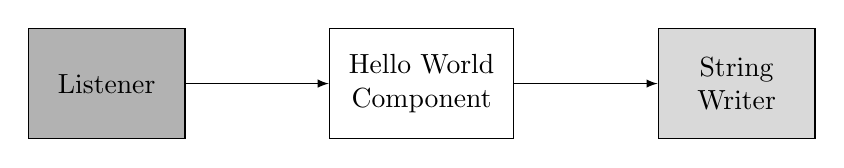
\begin{tikzpicture}[node distance = 2cm, auto]
    % Nodes
    \node [listener] (listener) {Listener};
    \node [component, right of=listener, text width=6em,, node distance=4cm] (hello) {Hello World Component};
    \node [writer, right of=hello, node distance=4cm] (writer) {String Writer};
    % Edges
    \path [line] (listener) -- (hello);
    \path [line] (hello) -- (writer);
\end{tikzpicture}
\caption[scale=1.0]{Hello world! server architecture.}
\label{fig:helloWorld}
\end{figure}

The \texttt{Listener} represents the 
part of the program that gets requests and feeds them to the network.
The \texttt{Hello World Component} inputs a client request from its input channel
and outputs the request together with the Hello World! string that should be 
used as a response to its output channel.
The \texttt{String Writer} writes the text response back to the client.

This is a good example of the basic components of the suggested framework.
We can call the three main parts the \texttt{Listener}, \texttt{Component} 
and \texttt{Writer}, where
the \texttt{Listener} catches the incoming requests and feeds them into the network,
the \texttt{Component} processes them and the \texttt{Writer} writes the generated result 
back to the client. That is \texttt{Listener} is the start and \texttt{Writer}
is the end of the server pipeline.

\subsection{File Server}
\label{sec:fileServer}
Architecture of a simple file server follows the architecture of the Hello world!
server introduced above. It consists of a \texttt{Listener}, which catches the requests,
\texttt{File Getter}, what is a function that gets the requested file (that is it
constructs the absolute path to the requested file and loads it into the memory) 
and finally there is a \texttt{File Writer}, which
writes the file to the client. The architecture is shown in Figure \ref{fig:fileServer}.
\begin{figure}[h]
\centering

\begin{tikzpicture}[node distance = 2cm, auto]
    % Nodes
    \node [listener] (listener) {Listener};
    \node [component, right of=listener, node distance=4cm] (getter) {File Getter};
    \node [writer, right of=getter, node distance=4cm] (writer) {File Writer};
    % Edges
    \path [line] (listener) -- (getter);
    \path [line] (getter) -- (writer);
\end{tikzpicture}
\caption[scale=1.0]{File server.}
\label{fig:fileServer}
\end{figure}

If we want to compress some subset of files, we can just add a \texttt{Splitter}
that sends files that are supposed to be compressed to a \texttt{Gzip Writer}, which
compresses the file and writes the result to the client. The rest of the files
will be passed to the standard \texttt{File Writer}. This architecture is shown in
Figure \ref{fig:fileServer2}.

\begin{figure}[h]
\centering
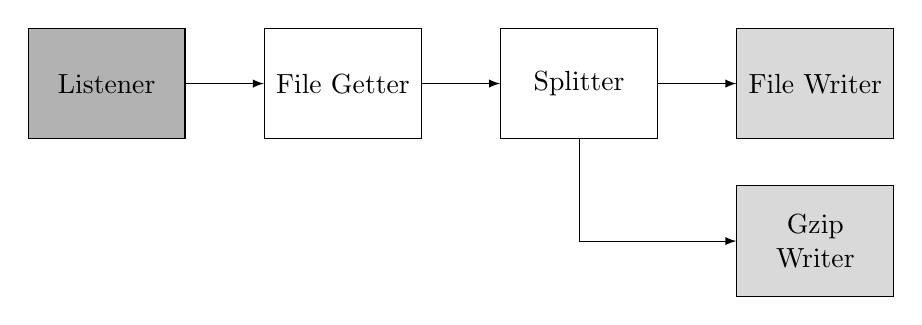
\begin{tikzpicture}[node distance = 2cm, auto]
    % Nodes
    \node [listener] (listener) {Listener};
    \node [component, right of=listener, node distance=3cm] (getter) {File Getter};
    \node [component, right of=getter, node distance=3cm] (splitter) {Splitter};
    \node [writer, right of=splitter, node distance=3cm] (fwriter) {File Writer};
    \node [writer, below of=fwriter] (gwriter) {Gzip Writer};
    % Edges
    \path [line] (listener) -- (getter);
    \path [line] (getter) -- (splitter);
    \path [line] (splitter) -- (fwriter);
    \path [line] (splitter) |- (gwriter);
\end{tikzpicture}
\caption[scale=1.0]{File server with compression.}
\label{fig:fileServer2}
\end{figure}

\subsection{Caching}
Suppose we have a worker component, which performs some expensive computation
and that we want to cache its output.
Using the proposed architecture we can just wrap the worker in a caching layer.
That is we only run the worker component if we don't have the result
in the cache, otherwise we just return the stored result. 
This design is show in Figure \ref{fig:caching}.

\begin{figure}[h]
\centering
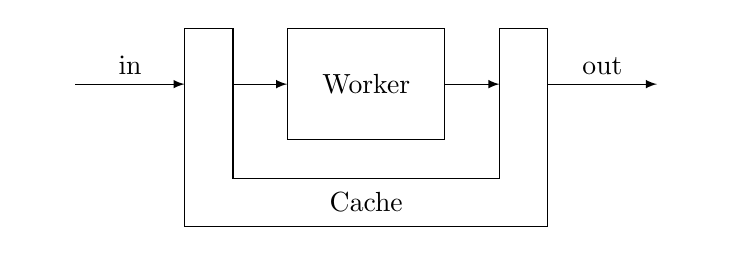
\begin{tikzpicture}[node distance = 1.5cm, auto,
    workerWidth/.style={text width=5em, text centered},
    workerHeight/.style={minimum height=4em},
    UWidth/.style={minimum width=0.6cm},
    UHeight/.style={minimum height=0.6cm}
    ]

    \node[component] (worker){Worker};
    \node [workerWidth, UHeight, below of=worker] (cache) {Cache};
    \node [UWidth, workerHeight, left of=worker, node distance=2cm] (left) {};
    \node [UWidth, workerHeight, right of=worker, node distance=2cm] (right) {};
    \node [UWidth, workerHeight, left of=left, node distance=2cm] (lleft) {};
    \node [UWidth, workerHeight, right of=right, node distance=2cm] (rright) {};

    \draw (left.north west) -- (left.west |- cache.south) -- (right.east |- 
          cache.south) -- (right.north east) -- (right.north west) -- 
          (right.west |- cache.north) -- (left.east |- cache.north) -- 
          (left.north east) -- cycle;

    \path[line] (lleft) edge node{in} (left);
    \draw[line] (left) -- (worker);
    \draw[line] (worker) -- (right);
    \path[line] (right) edge node{out} (rright);
\end{tikzpicture}\caption[scale=1.0]{Caching output of a worker component.}
\label{fig:caching}
\end{figure}

\subsection{Load Balancing}
If there is a lot of traffic in a certain part of the network we can
increase the throughput there
by creating multiple instances of the components in this part of 
the pipeline. The incoming request can then be passed to the component that is 
ready first. When the load in a given part of the pipeline decreases,
we can shut down the created components.

The benefit of the proposed architecture is that, we can do these adjustments
in runtime.
That is, based on current number of requests going through a certain part of 
the network we can decide to add or remove parts of the pipeline. This does not
have to be only adding components locally.
If we use channels over network then
we can connect to other servers and distribute the workload among them.
Hence we can start or shut down other servers based on the current traffic.
See Figure \ref{fig:loadBalancing} below.

\begin{figure}[h]
\centering
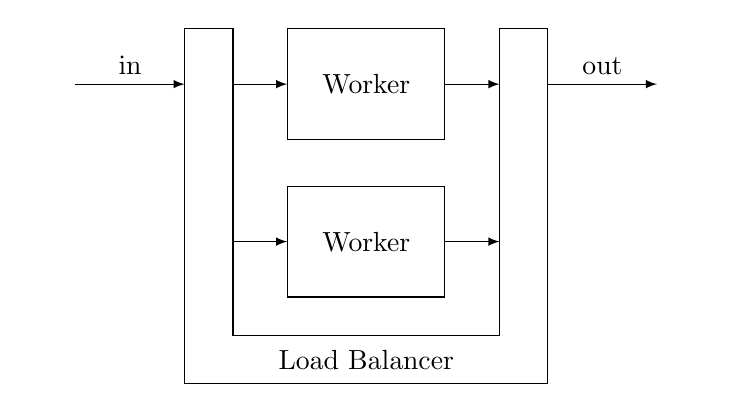
\begin{tikzpicture}[node distance = 1.5cm, auto,
    workerWidth/.style={text width=5em, text centered},
    workerHeight/.style={minimum height=4em},
    UWidth/.style={minimum width=0.6cm},
    UHeight/.style={minimum height=0.6cm}
    ]

    \node[component] (worker2){Worker};
    \node [component, below of=worker2, node distance=2cm] (worker) {Worker};
    \node [workerWidth, UHeight, below of=worker, text width=7em] (load) {Load Balancer};
    \node [UWidth, workerHeight, left of=worker, node distance=2cm] (left) {};
    \node [UWidth, workerHeight, left of=worker2, node distance=2cm] (left2) {};
    \node [UWidth, workerHeight, right of=worker, node distance=2cm] (right) {};
    \node [UWidth, workerHeight, right of=worker2, node distance=2cm] (right2) {};

    \node [UWidth, workerHeight, left of=left2, node distance=2cm] (lleft) {};
    \node [UWidth, workerHeight, right of=right2, node distance=2cm] (rright) {};

    \draw (left2.north west) -- (left2.west |- load.south) -- (right2.east |- 
          load.south) -- (right2.north east) -- (right2.north west) -- 
          (right2.west |- load.north) -- (left2.east |- load.north) -- 
          (left2.north east) -- cycle;

    \path[line] (lleft) edge node{in} (left2);
    \draw[line] (left) -- (worker);
    \draw[line] (left2) -- (worker2);
    \draw[line] (worker) -- (right);
    \draw[line] (worker2) -- (right2);
    \path[line] (right2) edge node{out} (rright);
\end{tikzpicture}\caption[scale=1.0]{
    Managing load in a given part of the network.
    One of the workers can be shut down or more workers can be added.
}
\label{fig:loadBalancing}
\end{figure}

\subsection{Comparison to Apache server configuration}
As noted before configuring an Apache serer can prove to be quite difficult.
Below in Figure \ref{fig:apache} is shown a part of a simple file server
configuration.
\begin{figure}[h]
\centering
\begin{lstlisting}[numbers=left]
Alias /project /path/to/project/

<Directory "/path/to/project/">
    Options Indexes
    AllowOverride None
    Order allow,deny
    Allow from localhost
    Require all granted
    AddOutputFilter DEFLATE py
</Directory>
\end{lstlisting}
\caption[scale=1.0]{Part of Apache configuration file for a file server.}
\label{fig:apache}
\end{figure}

The first line in the above configuration specifies that accessing URL 
path "/project" should point to the "/path/to/project/" directory.
Lines 3 to 10 specify who and how can access this directory.
The option \texttt{Options Indexes} indicates that if a client tries
to access a directory, then the server should list its contents.

\texttt{AllowOverride None} disables access to other directives when 
a file in the specified folder is accessed. Lines 6 to 8 specify that
anyone can access the directory. Finally, option 
\texttt{AddOutputFilter DEFLATE py} tells the server to compress
all python files, that is all files whose name ends with `.py'.

At first this does not look like a difficult configuration. However, 
one might argue that it is not as clear as the architecture proposed above,
as we are mixing different aspects of the server configuration in one place.
The main issue is that configuring more complex servers gets much more 
difficult very quickly. Furthermore if we want to serve dynamic content
we might need to use scripts written in other languages.

\subsection{Summary}
In this Chapter I described the conceptual architecture of the proposed
toolkit on a few simple examples. Then I showed configuration of a simple
Apache file server and contrasted this with my proposed architecture.
The next Chapter introduces the basic elements of my implementation.


%%%%%%%%%%%%%%%%%%%%%%%%%% Implementation %%%%%%%%%%%%%%%%%%%%%%%%%%%%%
\newpage
\section{Implementation}
\label{sec:impl}
In this Chapter I present basic elements of the \texttt{mpserver} toolkit
and how to work with them. The most important parts are the primitive types:
\texttt{Value}, \texttt{Component} and \texttt{Writer}.

\subsection{Values}
\texttt{Value} is an interface that represents the type of messages that are
passed between the components of the network. Its definition is shown
in Figure \ref{fig:Value} below.

\begin{figure}[h]
\centering
\begin{lstlisting}
type Value interface {
    //Public methods
    GetRequest() *http.Request
    GetResult() interface{}
    SetResult(interface{})
    SetResponseCode(int)
    SetResponseCodeIfUndef(int)
    SetHeader(string, string)

    // Private methods
    getResponseWriter() http.ResponseWriter
    getResponseCode() int
    writeHeader()
    write([]byte)
    close()
}
\end{lstlisting}
\caption[scale=1.0]{Declaration of the type \texttt{Value}.}
\label{fig:Value}
\end{figure}

Note that in Go only types, functions, constants and variables whose name
starts with a capital letter are exported from a package. Hence, anyone
using the package can only use the first 6 methods of the \texttt{Value}
interface.

The interface is implemented by a pointer to a private struct type shown in 
Figure \ref{fig:value}.
\newpage
\begin{figure}[h]
\centering
\begin{lstlisting}
type value struct {
    request *http.Request
    result interface{}

    responseCode int
    responseWriter http.ResponseWriter
    done chan<- bool
}
\end{lstlisting}
\caption[scale=1.0]{Declaration of a private type that implements the Value 
interface.}
\label{fig:value}
\end{figure}
Here:
\begin{itemize}
  \item \texttt{request} is a pointer to the HTTP request made by the 
        client implemented in the default http library. It can be accessed
        using the \texttt{GetRequest} method. 

  \item \texttt{result} is the result computed so far (initially \texttt{nil}). This is
        of type \texttt{interface\{\}} which is implemented by any type.
        Hence, values of all types can be stored there. This field can be
        accessed and changed using the \texttt{GetResult} and \texttt{SetResult}
        methods respectively.
  
  \item \texttt{responseCode} is the HTTP response code that should be 
        returned to the client. The default value of this field is $-1$,
        which indicates that the \texttt{responseCode} hasn't been set yet. 
        It can be set using the \texttt{SetResponseCode} or 
        \texttt{SetResponseCodeIfUndef} methods, where the second method only
        makes a change in case the response code has not been set yet. The value
        of the response code can be retrieved using the \texttt{getResponseCode}
        method inside the package. This is only used by a 
        \texttt{Writer} type that is introduced later.

  \item \texttt{responseWriter} is an object that writes the response back 
        to the client. Again only \texttt{Writers} use this field. They
        can retrieve it using \texttt{getResponseWriter} method. 
        Alternatively, they can use the \texttt{write\-Header}
        and \texttt{write} methods to access the field indirectly.
        These methods write the headers and 
        the body of the response to the client respectively.

  \item \texttt{done} is a signaling channel. Signal is sent on this channel,
		after the response is written at the end of the pipeline using the 
        \texttt{close} method. This allows the connection to the client to 
        be closed after the result is written.
\end{itemize}
Note that all methods related to writing the response back to the client
are private to the package. This is to ensure correct behavior, as otherwise
these methods could be accessed by users of the package in any part of the 
network, what could lead to panic.

\subsection{Components}
This section introduces the \texttt{Component} type and then shows how we can simply
create components. Afterwards it presents a way how multiple components can
be combined to form a linear pipeline. The sections ends with a description
of a component generator that implements simple load balancing among
multiple components.

\subsubsection{The Component type}
Component is a generic part of the pipeline with an input and an output channel.
It processes the values provided on input channel and outputs the results
on the output channel. The type \texttt{Component} is defined as follows:
\begin{lstlisting}
type Component func (in <-chan Value, out chan<- Value)
\end{lstlisting}
Every component should satisfy the following conditions:
\begin{itemize}
    \item When run a component should eventually read all values that are
          written to its input channel.

    \item Every value that a component reads from its input channel
          should be written to its output channel after the value was processed
          and possibly modified. This ensures that every request gets a response.

    \item A component can terminate only when its input channel is closed. 
          Before terminating, the component should close its output channel.
          This ensures termination of any components further down the network.

    \item Component can only close its output channel and it can only do so
    	    after its input channel have been closed. It should never attempt
          to close the input channel as this will likely result in a panic.
\end{itemize}

\subsubsection{Making Components}
To simplify the construction of components, so that they adhere to 
the above specification the package provides a helper function that 
constructs a component using a function that takes a \texttt{Value} object 
and processes it. The \texttt{Value} can be modified by the function as it is 
implemented by a pointer type. The function has the following signature:
\begin{lstlisting}
type ComponentFunc func (val Value)
\end{lstlisting}
This represents a transition function that is applied to input values
to produce output values.
The implementation of the described component generator is shown in 
Figure \ref{fig:MakeComponent} below.
\begin{figure}[h]
\centering
\begin{lstlisting}
func MakeComponent(f ComponentFunc) Component {
    return func (in <-chan Value, out chan<- Value) {
        for val := range in {
            f(val); out <- val
        }
        close(out)
    }
}
\end{lstlisting}
\caption[scale=1.0]{Declaration of the \texttt{MakeComponent} function.}
\label{fig:MakeComponent}
\end{figure}

Here the for loop reads values from the input channel and assigns them
to the variable \texttt{val} while the input channel is open. Then the 
the function \texttt{f} is applied to this value and finally the value is outputted.
Afterwards, the component waits for another value. When the input channel
is closed the loop terminates. Afterwards, the component closes its output channel
and terminates.

\subsubsection{Constant Component}
Constant Component is a simple component generator that takes a value \texttt{c}
of any type and returns a component that writes \texttt{c} to the result field of 
all input values and then outputs them. It's definition using the 
\texttt{MakeComponent} generator is shown in Figure 
\ref{fig:ConstantComponent} below.
\begin{figure}[h]
\centering
\begin{lstlisting}
func ConstantComponent(c interface{}) Component {
    return MakeComponent(func (val Value) {
        val.SetResult(c)
    })
}
\end{lstlisting}
\caption[scale=1.0]{Declaration of constant component generator.}
\label{fig:ConstantComponent}
\end{figure}

\subsubsection{Linking components}
The library also provides a component generator \texttt{LinkComponents} that takes 
any number of components and returns a component that behaves as their 
linear combination. That is as a pipeline constructed from these components 
in the order in which they are provided. Its signature is shown below.
\begin{lstlisting}
func LinkComponents(components ...Component) Component
\end{lstlisting}
The subcomponents are linked and run when the combined component is run. 
The last of the provided components is run in the goroutine in which
the combined component was run.

\subsubsection{Simple Load Balancing}
To support running the same component with the same input and output 
channels multiple times the toolkit provides \texttt{StaticLoadBalancer}.
Note that this is possible as channels in go are many-to-many.
\texttt{StaticLoadBalancer} is a component generator that takes a worker 
component and number $n$ and returns a component that when run starts 
$n$ instances of the worker component. 

The case with $n=3$ in a simple pipeline is shown in Figure \ref{fig:slbEx} below. 
In order to support clean shutdown of the combined component, the load balancer uses 
wrappers (U shaped components in the diagram) around workers and a component that 
forwards incoming values to the workers. When input channel of the forwarding
component is closed it sends a signal to the component wrappers on shut 
down channels (dashed arrows in the diagram). The wrappers then close
the channels to the workers, which will force the workers to terminate.
Finally the distributor closes the output channel of the whole component
and then the termination signal propagates further down the network.

\begin{figure}[h]
\centering
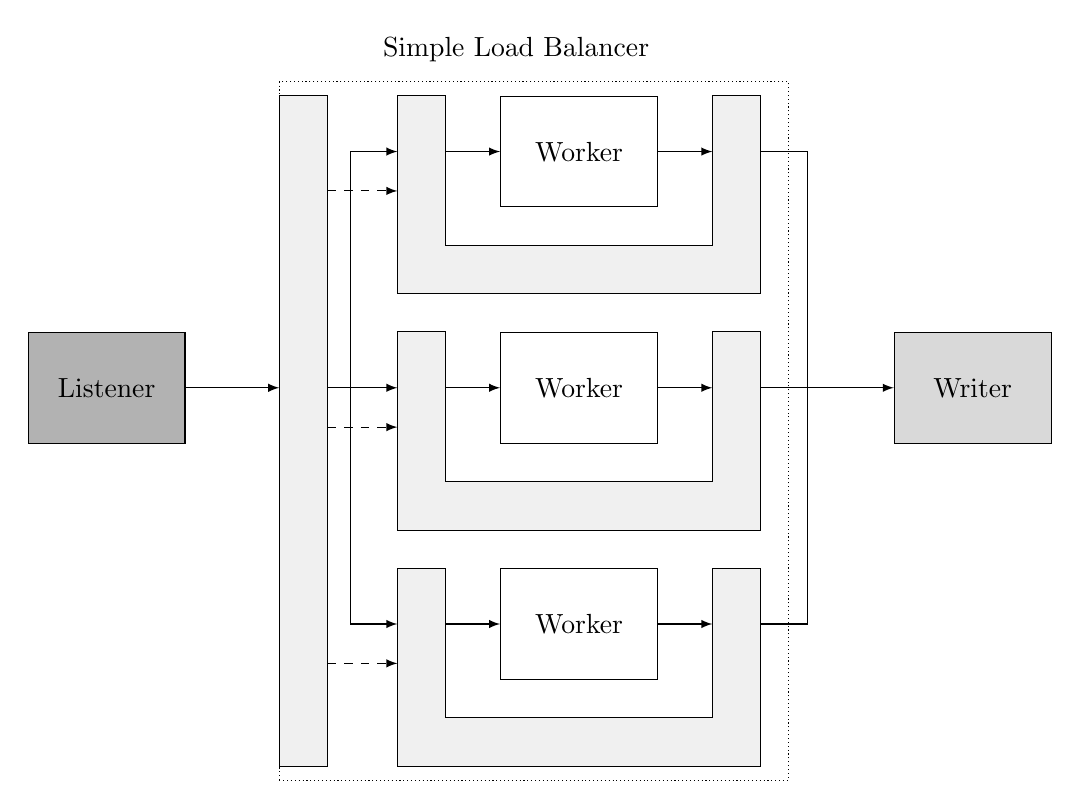
\begin{tikzpicture}[node distance = 1.5cm, auto,
    workerWidth/.style={text width=5em, text centered},
    workerHeight/.style={minimum height=4em},
    UWidth/.style={minimum width=0.6cm},
    UHeight/.style={minimum height=0.6cm}
    ]
    % Nodes
    \node [component] (worker1) {Worker};
    \node [workerWidth, UHeight, below of=worker1] (passer1) {};
    \node [workerWidth, UHeight, above of=worker1] (passer2) {};
    \node [component, above of=passer2] (worker2) {Worker};
    \node [component, below of=passer1] (worker3) {Worker};
    \node [workerWidth, UHeight, below of=worker3] (passer3) {};
    \node [above of=worker2, node distance=1.3cm, xshift=-0.8cm] {Simple Load Balancer};

    % Left
    \node [UWidth, workerHeight, left of=worker1, node distance=2cm] (left1) {};
    \node [UWidth, workerHeight, left of=worker2, node distance=2cm] (left2) {};
    \node [UWidth, workerHeight, left of=worker3, node distance=2cm] (left3) {};

    \node [UWidth, workerHeight, left of=left1, node distance=1.5cm] (lleft1) {};
    \node [UWidth, workerHeight, left of=left2, node distance=1.5cm] (lleft2) {};
    \node [UWidth, workerHeight, left of=left3, node distance=1.5cm] (lleft3) {};

    \draw[fill=gray!12] (lleft2.north west) -- (lleft2.west |- passer3.south) --
          (lleft2.east |- passer3.south) -- (lleft2.north east) --
          cycle;

    % Right
    \node [UWidth, workerHeight, right of=worker1, node distance=2cm] (right1) {};
    \node [UWidth, workerHeight, right of=worker2, node distance=2cm] (right2) {};
    \node [UWidth, workerHeight, right of=worker3, node distance=2cm] (right3) {};

    \draw[fill=gray!12] (left1.north west) -- (left1.west |- passer1.south) -- 
          (right1.east |- passer1.south) -- (right1.north east) -- 
          (right1.north west) -- (right1.west |- passer1.north) -- 
          (left1.east |- passer1.north) -- (left1.north east) -- cycle;
    \draw[fill=gray!12] (left2.north west) -- (left2.west |- passer2.south) -- 
          (right2.east |- passer2.south) -- (right2.north east) -- 
          (right2.north west) -- (right2.west |- passer2.north) -- 
          (left2.east |- passer2.north) -- (left2.north east) -- cycle;
    \draw[fill=gray!12] (left3.north west) -- (left3.west |- passer3.south) -- 
          (right3.east |- passer3.south) -- (right3.north east) -- 
          (right3.north west) -- (right3.west |- passer3.north) -- 
          (left3.east |- passer3.north) -- (left3.north east) -- cycle;

    \node [listener, left of=left1, node distance=4cm] (listener) {Listener};
    \node [writer, right of=right1, node distance=3cm] (writer) {Writer};
    % Edges
    \path [line] (listener) -- (lleft1);
    \path [line] (lleft1) -- (left1);
    \path [line] ($ (lleft1) !.4! (left1) $) |- (left2);
    \path [line] ($ (lleft1) !.4! (left1) $) |- (left3);

    \path [line, dashed,transform canvas={shift={(0,-0.5)}}] (lleft1) -- (left1);
    \path [line, dashed,transform canvas={shift={(0,-0.5)}}] (lleft2) -- (left2);
    \path [line, dashed,transform canvas={shift={(0,-0.5)}}] (lleft3) -- (left3);

    \path [line] (left1) -- (worker1);
    \path [line] (left2) -- (worker2);
    \path [line] (left3) -- (worker3);

    \path [line] (worker1) -- (right1);
    \path [line] (worker2) -- (right2);
    \path [line] (worker3) -- (right3);
    \path [line] (right1) -- (writer);
    \path [draw] (right2) -| ($ (right1) !.3! (writer) $);
    \path [draw] (right3) -| ($ (right1) !.3! (writer) $);
    \node[xshift=0.5em, draw, densely dotted, minimum width=18em, inner sep=0.5em,fit=(right2) (right3) (lleft2) (lleft3) (passer3)] {};
\end{tikzpicture}
\caption[scale=1.0]{Simple server example showing usage of \texttt{StaticLoadBalancer}.}
\label{fig:slbEx}
\end{figure}

This combined component allows multiple requests to be processed by the worker
components at the same time and this in turn allows faster requests to 
overtake slower requests in the pipeline. The worker component can represent
a simple computation done locally or they can connect to other servers
and perform expensive computation there. More advanced version of load 
balancing component is introduced in the next chapter.

\newpage
\subsection{Writers}
In this section I introduce the \texttt{Writer} type, which acts as the end of the 
pipeline. Then I present a way how to create custom writers.
\subsubsection{Writer type}
Writer is the end of the pipeline which writes results back to the client.
The type \texttt{Writer} is defined as follows:
\begin{lstlisting}
type Writer func (in <-chan Value)
\end{lstlisting}
It is a function with only an input channel.
Every writer satisfies the following specification.
\begin{itemize}
    \item When run a writer eventually reads all values that are written 
          to its input channel.

	\item For every value that is input any writer behaves as follows. 
        It firstly checks if the result field contains the expected type. 
        If that is the case, it first writes the headers and then
        the body of the response using the \texttt{writeHeader} and
        \texttt{write} methods of the value respectively. 
        Afterwards it closes the connection for the value and using 
        the \texttt{close} method. If the value in the result 
        field has an incorrect type, the writer writes an appropriate 
        error message to the client and closes the connection for the value. 

	\item The writer terminates when its input channel is closed.
\end{itemize}
The package provides writers for writing string, json, file, error and many
other types of responses. There is also a writer generator for static
load balancing similar to the one for components. It's implementation
is significantly simpler as we don't have to forward the processed
values further down the network. Note that components
combined with writers appear like a single writer. Hence, we can use the
load balancers for writers to manage a more complex part the network.

\subsubsection{Making Writers}
As noted before the methods for writing responses from \texttt{Values}
back to the client cannot be used outside of the package. To allow
for construction of custom writers the package provides writer generator
component similar to the \texttt{MakeComponent} function. It uses 
functions with the following signature to generate the writers.
\begin{lstlisting}
type WriterFunc func (val Value) ([]byte, error)
\end{lstlisting}
This function should set headers and convert the provided value into 
a slice\footnote{``Slice is a dynamically-sized, flexible view into the elements 
of an array.''\cite{tour}} of bytes or return an error in case it 
is provided with a 
wrong input. The implementation of the writer generator itself is shown
in Figure \ref{fig:MakeWriter} below.
\begin{figure}[h]
\centering
\begin{lstlisting}
func MakeWriter(writerFunc WriterFunc) Writer {
    return func (in <-chan Value) {
        for val := range in {
            resp, err := writerFunc(val)

            if (err == nil) {
                // Write the response
                val.SetResponseCodeIfUndef(http.StatusOK)
                val.writeHeader()
                val.write(resp)
                val.close()
            } else {
                writeError(val, err)
            }
        }       
    }
}
\end{lstlisting}
\caption[scale=1.0]{Implementation of writer generator.}
\label{fig:MakeWriter}
\end{figure}

The generated writer runs the provided \texttt{writerFunc} for every value 
that is inputted. If the function returns an error it writes the error 
back to the client using the \texttt{writeError}\footnote{See Appendix 
\ref{sec:writer.go} for the implementation.} function. Otherwise, it 
writes the headers and the body of the response to the client and then 
closes the connection. (The \texttt{writeError} does this for the error
results).

\subsection{Splitter and Collector}
In this section I introduce a way to split a stream of incoming values into
multiple streams of values that go into different parts of the network
using very flexible rules for splitting. Then I present a way how to
safely combine multiple streams into one.

\subsubsection{Conditions}
Condition type is defined as follows:
\begin{lstlisting}
type Condition func (val Value) bool
\end{lstlisting}
It is a just function that takes a value and returns a boolean.
The function shouldn't change the provided value.

\subsubsection{Splitter}
Conditions are used in Splitter, which is a component with the 
following signature:
\begin{lstlisting}
func Splitter(in <-chan Value, defOut chan<- Value, 
			  outs []chan<- Value, conds []Condition)
\end{lstlisting}
It takes an input channel, default output channel, a slice of output channels 
and a slice of conditions.
The number of output channels and the number of conditions should be the same.
For every input value the Splitter evaluates the conditions from first to last.
When a condition returns \texttt{true} the value is written to a 
corresponding output channel 
and the processing of the current value terminates. If all conditions 
return \texttt{false} then the value is written to the default output channel.

\subsubsection{Error Splitter}
The package also implements a special splitter that redirects error messages
to a special error channel and sends all other messages to the default output 
channel. This is used to avoid sending error values to 
any other type of writer than the error writer. If we allowed this, then
all errors will only show that a particular writer got a wrong input.
The signature of the \texttt{ErrorSplitter} function is shown below.
\begin{lstlisting}
func ErrorSplitter(in <-chan Value, defOut chan<- Value, 
                                    errChan chan<- Value)
\end{lstlisting}

\subsubsection{Collector}
Collector is a component whose behavior is the opposite of the behavior 
of a splitter. It gets multiple input channels
and forwards their outputs to a single output channel. Now as channels
in go are many-to-many we could just use a single channel to which
multiple components would output their values. 

However, when we shutdown
one of the components, this component will close the output channel
what will cause panic next time one of the other components tries to write
to it. Now, \texttt{Collector} only closes its output channel, when
all of its input channels have been closed, thus avoiding the problem 
described above. It is acceptable to just use a single channel instead of
the collector component, if we don't intend to shut down the network.
The type signature of the \texttt{Collector} is show below.
\begin{lstlisting}
func Collector(ins []<-chan Value, out chan<- Value)
\end{lstlisting}


\subsection{Summary}
In this Chapter I introduced the basic elements of the toolkit. This 
is enough to implement some simple serves. The next section introduces
more advanced components that allow more complex behaviors.



%%%%%%%%%%%%%%%%%%%%%%%%%% Implementation 2 %%%%%%%%%%%%%%%%%%%%%%%%%%%
\newpage
\section{Advanced component generators}
\label{sec:impl2}
In this section I introduce more advanced component generators for caching,
session management, load balancing, network communication and error handling.

\subsection{Storage}
\texttt{Storage} is an interface representing thread safe mapping from string keys
to values of any type. Its definition is shown in Figure \ref{fig:Storage} below.
\begin{figure}[h]
\centering
\begin{lstlisting}
type Storage interface {
    Get(string) (interface{}, bool)
    Set(string, interface{})
    Remove(string)
    CompareAndRemove(string, interface{}) bool
    Keys() []string
}
\end{lstlisting}
\caption[scale=1.0]{Declaration of the \texttt{Storage} interface.}
\label{fig:Storage}
\end{figure}
The package provides a default implementation of this interface that
stores the data in memory using (with minor modifications) sharded concurrent map implementation
by Or Hiltch\footnote{Code available at \url{https://github.com/orcaman/concurrent-map}}.
If a developer wants to store the values in the 
database instead, they can provide their own implementation of the 
\texttt{Store} interface
and use any component that uses the storage the same way as before.
This makes the components that use the storage highly configurable.

\subsection{States and Session Management Component}
\subsubsection{States}
\label{sec:state}
\texttt{State} is an interface defined in Figure \ref{fig:State}.
\begin{figure}[h]
\centering
\begin{lstlisting}
type State interface {
    Next(val Value) (State, error)
    Terminal() bool
    Result() Any
}
\end{lstlisting}
\caption[scale=1.0]{Declaration of the State interface.}
\label{fig:State}
\end{figure}
The expected behavior of the member functions is as follows:
\begin{itemize}
	\item The \texttt{Next} function returns the next state when provided 
          with a value.
	\item The \texttt{Terminal} function indicates whether the current 
          state is a terminal state.
	\item The \texttt{Result} function returns the result that possibly 
          after further processing should be returned to the client.
\end{itemize}

\subsubsection{Session Management}
\texttt{SessionManager} is a component generator with the following signature:
\begin{lstlisting}
func SessionManager(store Storage, initial State, 
                seshExp time.Duration, useCleaner bool) Component
\end{lstlisting}
Its arguments are a storage object to be used, an initial state for each session,
a session expiration time and a boolean indicating whether expired
entries should be automatically removed from the map.
The returned component behaves as a session manager. 
Its behavior is described below.

The component stores a mapping from session ids to current state of the session.
Every new request gets assigned a unique session id. Then a current state
of the session is generated from the initial state using the provided
value. Afterwards a mapping from the generated id to the current state
is stored. The result of the call to the \texttt{Result} function on the
current state with the provided value is then sent down the pipeline and
client response is generated from it.

When a request with set `Session-Id` header comes in, the component gets the current 
state for the session and gets the next state for it based on the provided value.
The mapping is then updated with the new state and the result from the new state
is passed down the pipeline.

When a session reaches a Terminal state, the session id is removed from the map
and the final result is outputted.

The states in the mapping are timestamped and are removed from the map after
the session expiration time, if the session haven't finished before that.

% More hype
The abstraction using states allows the users of the package to implement the
logic for the session, independently of the session management part.

\subsection{Caching}
\texttt{CacheComponent} is a component generator with the following signature:
\begin{lstlisting}
func CacheComponent(cache Storage, worker Component, 
            expiration time.Duration, useCleaner bool) Component
\end{lstlisting}
The returned component behaves as follows:
\begin{itemize}
	\item When a value is input that the component hasn't seen before, then
		  the value is passed to the provided worker and the result is stored in
		  a map.
	\item When the component gets a previously seen value, it returns the value
		  stored in the map, if it hasn't expired yet. If it expired, then the component
		  treats it as a new value.
	\item Expired values are regularly deleted from the map if the useCleaner
          option is set to \texttt{true}.
\end{itemize}

For the generated component to function properly, the worker must output
a value for every value that is sent to it. This is one of the conditions
that any component must satisfy, so this shouldn't be an issue.

\subsection{Dynamic Load Balancing}
\texttt{DynamicLoadBalancer} is a component generator whose signature is
shown below. Its architecture is similar
to that of the \texttt{StaticLoadBalancer}.
\begin{lstlisting}
func DynamicLoadBalancer(addTimeout, removeTimeout time.Duration, 
        worker Component, maxWorkers int) Component
\end{lstlisting}
The returned component has an array of workers which can be easily shut down.
The initial number of workers is 1. 
For every input value, the component behaves as follows:
\begin{itemize}
	\item It tries to send the value to the workers, if this is not successful, 
		  before the \texttt{addTimeout}, then the component creates a new worker
          if the current number of workers is smaller than \texttt{maxWorkers}.
          Then the component tries to send the value to the workers again. This will 
          be successful in case a worker was added because there is at least one 
          worker that is not busy.

	\item The workers send their results further down the pipeline.

	\item If there are no incoming values for duration equal to the 
          \texttt{removeTimeout}, then the component shuts down one 
          of the workers, if there is more than one worker.

	\item When the input channel of the component is closed, then the load balancer 
          shuts down all the workers and afterwards closes its output channel and
          terminates.
\end{itemize}
There are a lot of other possible load balancing strategies. 
Implementing them should be a simple modification of the existing code.
Note that this is very powerful concept as it can also be used to share
the load between multiple servers and turn them on or shut them down as
required (here using a different strategy might be preferred). There is
also a similar dynamic load balancer for writers.

\subsection{Error handling}

\subsubsection{Error Passer}
As a lot of components expect an input of a certain type, their execution
might end with an error if they are provided with an error result from
the previous component. This would make debugging very hard. Hence, the 
package provides the following component wrapper, that allows error messages
to bypass a component. The signature of this wrapper is shown below.
\begin{lstlisting}
func ErrorPasser(worker Component) Component
\end{lstlisting}
The inner design of the generated component is shown in Figure 
\ref{fig:errPasserDiag}. The behavior of the generated component 
can be described as follows:
\begin{itemize}
	\item For every input value it checks whether the result is an error
		  and if that is the cases it just outputs the value.
	\item If the result of the input value is not an error, then the component
		  passes the value to the worker, which after processing it passes 
		  it further down the pipeline.
\end{itemize}

\begin{figure}[h]
\centering
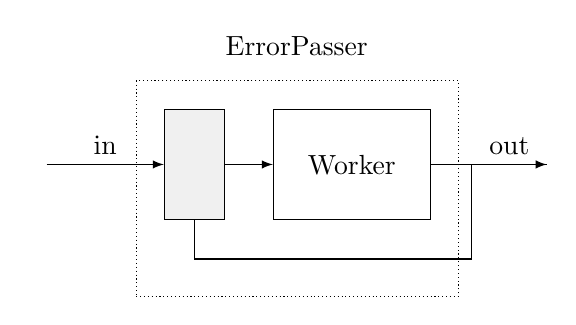
\begin{tikzpicture}[node distance = 2cm, auto]
    % Nodes
    \node[component, fill=gray!12, text width=1.5em] (passer) {};
    \node[component, right of=passer] (worker) {Worker};
    \node[above of=worker, node distance=1.5cm, xshift=-0.7cm](name){ErrorPasser};
    \node[text width=2em, right of=worker] (right) {};
    \node[below of=worker, node distance=1.2cm] (lineh) {};
    \node[left of=passer] (left) {};

    % Edges
    \path[line] (left) edge node {in} (passer); 
    \path (right.west) edge node {out} (right.east);
    \path[line] (right.west) -- (right.east);
    \path[line] (passer) -- (worker);
    \path[draw] (worker) -- (right);
    \path[draw] (passer.south) |- (lineh.east);
    \path[draw] (lineh.east) -| (right.west);
    \node[draw, densely dotted, inner sep=1em,
          fit=(passer) (worker) (lineh)] {};
\end{tikzpicture}
\caption[scale=1.0]{Inner design of the components generated with
  \texttt{ErrorPasser}.}
\label{fig:errPasserDiag}
\end{figure}

\subsubsection{Panic handling}
If we use a component which might cause panic, this will crash the whole
server when the panic occurs. Hence, the package provides the 
\texttt{PanicHandler}. The signature of this wrapper is shown 
below.
\begin{lstlisting}
func PanicHandler(worker Component) Component
\end{lstlisting}
It takes a component that can cause panic and returns a component the 
behaves as follows:
\begin{itemize}
	\item It passes every input value to the worker, gets the result 
        from it and then passes the result further down the pipeline.
	\item In case the worker crashes, that is it causes panic, the component 
        writes an error as a result for the value that caused the crash 
        and then restarts the worker.
	\item The component can itself cause a panic if the worker closes its 
        input channel, or if it closes its output channel before its input 
        channel is closed. That is if the worker violates the contract
        for components.
\end{itemize}

\subsection{Network Components}
In this section I present a component generator that can make network
requests. Then I introduce a helper component that alters incoming 
requests, so that they can be performed again using a different host
and a component that processes HTTP responses. Finally, I show how
can these components be plugged together to act as a proxy server. 

\subsubsection{Network Component}
Network Component is a component generator with the following signature:
\begin{lstlisting}
func NetworkComponent(client *http.Client) Component
\end{lstlisting}
It takes a single parameter, which is an http client.
The generated component for each input value makes an http request,
taken from the Result field of the value, using the provided http client.
If there is no request in the Result field or the request fails, then
the component returns an appropriate error. The behavior of the generated 
component is described in Figure \ref{fig:networkComp} below.

\begin{figure}[h]
\centering
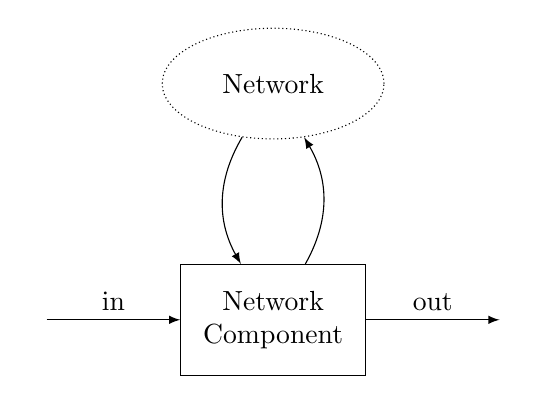
\begin{tikzpicture}[node distance = 2cm, auto]
    % Nodes
    \node [component, densely dotted, ellipse] (internet) {Network};
    \node [component, text width=6em, below of=internet, node distance=3cm] (network) {Network Component};
    \node [left of=network, node distance = 3cm] (in) {};
    \node [right of=network, node distance = 3cm] (out) {};
    % Edges
    \path[line] (network) edge [bend right] (internet);
    \path[line] (internet) edge [bend right] (network);
    \path[line] (in) edge node {in} (network);
    \path[line] (network) edge node {out} (out);
\end{tikzpicture}
\caption[scale=1.0]{Design of the network component.}
\label{fig:networkComp}
\end{figure}

Note that the result of the request is fetched in the goroutine where the
component runs. Hence, slow requests might block the pipeline. To avoid
this behavior \texttt{NetworkComponent} is usually used together with one
of the load managers.

\subsubsection{Request Copier}
Request Copier is a component generator with the following signature:
\begin{lstlisting}
func RequestCopier(scheme, host string) Component
\end{lstlisting}
It takes string parameters scheme (e.g. http) and host (e.g. www.google.com) 
and returns a component that for each input value copies the Request made 
by the client to the Result field and updates it with the given scheme and 
path and then outputs this value.

\subsubsection{Response Processor}
The \texttt{Response} type of the \texttt{mpserver} is defined a struct
that is shown in Figure \ref{fig:Response}.
\begin{figure}[h]
\centering
\begin{lstlisting}
type Response struct {
		Header http.Header
		Body []byte
}
\end{lstlisting}
\caption[scale=1.0]{Declaration of type Response.}
\label{fig:Response}
\end{figure}

It holds the headers and body of an http response. The difference between
this definition and the definition in the default \texttt{http} package is that
the body of my \texttt{Response} is a slice of bytes. 
That is the body have already been
read and the connection to the server has been closed.

The \texttt{ResponseProcessor} is a component that for each input value
looks if the provided result is the default \texttt{http} Response. 
If that is the case,
then it reads the response and transfers it to \texttt{mpsever Response} 
type, which it
then writes to the result field and outputs the value. If no response
is provided, then the component outputs an appropriate error.

To use this component after the \texttt{NetworkComponent}, 
the \texttt{ResponseProcessor}
should be wrapped in an error passing component, so that when the\\
\texttt{NetworkComponent} fails, then the response processor won't have to do
any work.

\subsubsection{Proxy Component}
Proxy component is a combination of \texttt{RequestCopier}, 
\texttt{NetworkComponent} 
and \texttt{ResponseProcessor} in a linear pipeline. It acts as a proxy server
in the following sense. It forwards the provided request to the specified
host and then reads and outputs the response. 

All components are wrapped
in an \texttt{ErrorPasser} to avoid doing unnecessary work and to make the component
more robust. Furthermore, the linear combination of all the components is wrapped in 
\texttt{DynamicLoadBalancer} to make the whole component more 
responsive. The implementation is shown in Figure \ref{fig:ProxyComp} below.

\begin{figure}[h]
\centering
\begin{lstlisting}
func ProxyComponent(scheme, host string, client *http.Client, 
        addTime, removeTime time.Duration, nReq int) Component {
    return DynamicLoadBalancer(
        addTimeout, removeTimeout,
        LinkComponents(
            ErrorPasser(RequestCopier(scheme, host)),
            ErrorPasser(NetworkComponent(client)),
            ErrorPasser(ResponseProcessor)),
        nReq)
}
\end{lstlisting}
\caption[scale=1.0]{Declaration of Proxy Component generator.}
\label{fig:ProxyComp}
\end{figure}
\subsection{Summary}
In this section I introduced more advanced component wrappers and generators
and described how to use them. The next section shows a few example
servers implemented using my toolkit.



%%%%%%%%%%%%%%%%%%%%%%%%%%%%%% Examples %%%%%%%%%%%%%%%%%%%%%%%%%%%%%%%
\newpage
\section{Examples}
\label{sec:examples}
\subsection{Hello world! server}
Figure \ref{fig:HelloWorldImpl} shows the Implementation of the Hello World!
server described in section \ref{sec:helloWorld}.
It's a direct translation of the diagram shown in Figure \ref{fig:helloWorld}.

The Listener corresponds to the call of \texttt{mpserver.Listen} function.
Hello world Component translates into an instance of \texttt{ConstantComponent}
and String Writer is the writer in the package with the same name.
We plug these together using two channels, start the component and writer 
and then start the server itself.

\begin{figure}[h]
\centering
\lstinputlisting{../examples/helloServer/helloServer.go}
\caption[scale=1.0]{Implementation of the Hello World! server.}
\label{fig:HelloWorldImpl}
\end{figure}

\newpage
\subsection{File server}
Figure \ref{fig:FileServerImpl} shows the implementation of a simple 
file server that compresses all '.go' files. It is almost a direct translation
of the diagram shown in figure \ref{fig:fileServer2} in section \ref{sec:fileServer}.
However, here the File Getter is composed of two parts, which are \texttt{PathMaker}
and \texttt{FileComponent}. The \texttt{PathMaker} firstly strips a given
prefix from the request path and then prepends a provided directory name to 
the result. The \texttt{FileComponent} tries to open a file at a path 
provided in the result field of the incoming value. Other modifications
are the addition of the \texttt{ErrorWriter} and the channel going to it from
the \texttt{Splitter}.
This path is used when a non existent file is requested by the client.
Otherwise '.go' files goes to the \texttt{GzipWriter} and all other files to 
the standard \texttt{FileWriter}.
The diagram that represents this server is shown in 
Figure \ref{fig:fileServer3}.

\begin{figure}[h]
\centering
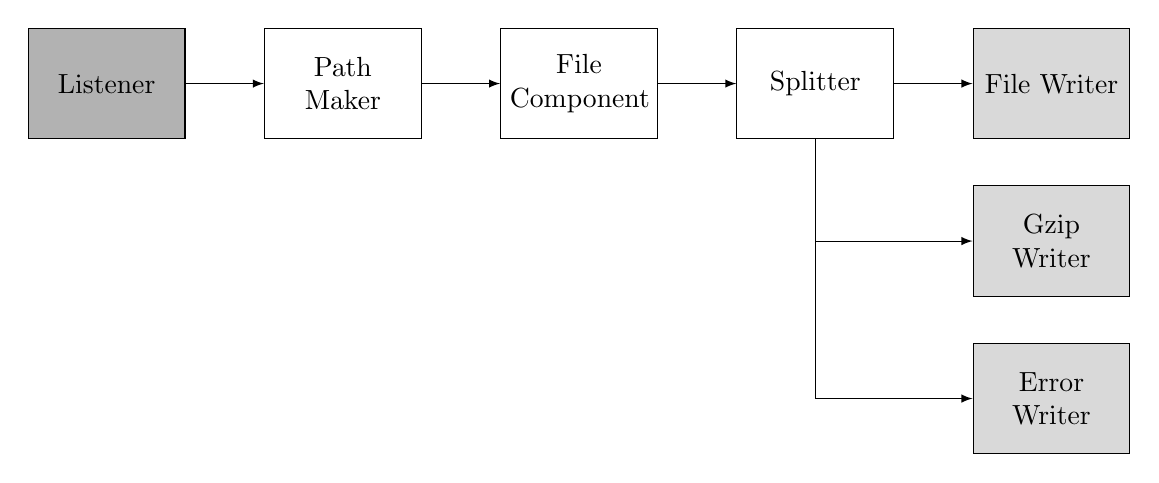
\begin{tikzpicture}[node distance = 2cm, auto]
    % Nodes
    \node [listener] (listener) {Listener};
    \node [component, right of=listener, node distance=3cm] (maker) {Path Maker};
    \node [component, right of=maker, node distance=3cm] (comp) {File Component};
    \node [component, right of=comp, node distance=3cm] (splitter) {Splitter};
    \node [writer, right of=splitter, node distance=3cm] (fwriter) {File Writer};
    \node [writer, below of=fwriter] (gwriter) {Gzip Writer};
    \node [writer, below of=gwriter] (ewriter) {Error Writer};
    % Edges
    \path [line] (listener) -- (maker);
    \path [line] (maker) -- (comp);
    \path [line] (comp) -- (splitter);
    \path [line] (splitter) -- (fwriter);
    \path [line] (splitter) |- (gwriter);
    \path [line] (splitter) |- (ewriter);
\end{tikzpicture}
\caption[scale=1.0]{File server with compression and error handling.}
\label{fig:fileServer3}
\end{figure}

\begin{figure}
\lstinputlisting{../examples/fileServer/fileServer.go}
\caption[scale=1.0]{Implementation of a File Server that compresses go files.}
\label{fig:FileServerImpl}
\end{figure}

\newpage
\subsection{Proxy server}
A simple proxy server can be represented by a diagram shown in Figure
\ref{fig:proxyServer} below.
\begin{figure}[h]
\centering
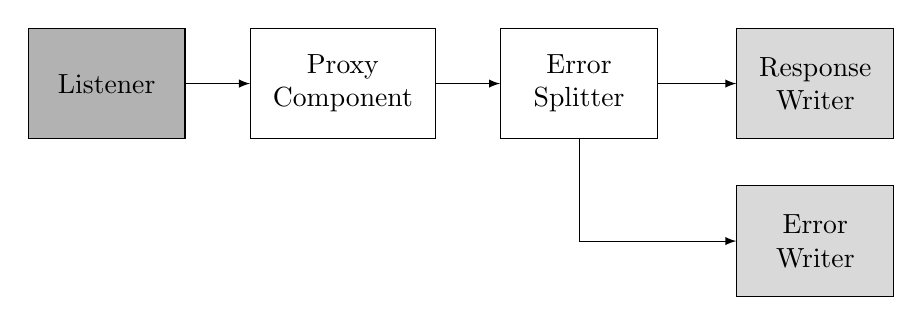
\begin{tikzpicture}[node distance = 2cm, auto]
    % Nodes
    \node [listener] (listener) {Listener};
    \node [component, text width=6em, right of=listener, node distance=3cm] (proxy) {Proxy Component};
    \node [component, right of=proxy, node distance=3cm] (splitter) {Error Splitter};
    \node [writer, right of=splitter, node distance=3cm] (rwriter) {Response Writer};
    \node [writer, below of=rwriter] (ewriter) {Error Writer};
    % Edges
    \path [line] (listener) -- (proxy);
    \path [line] (proxy) -- (splitter);
    \path [line] (splitter) -- (rwriter);
    \path [line] (splitter) |- (ewriter);
\end{tikzpicture}
\caption[scale=1.0]{Simple proxy server.}
\label{fig:proxyServer}
\end{figure}

Now to increase throughput of this server I propose wrapping the Proxy
Component in a Static Load Balancer. However, now the number of writers
will be the limiting factor, so I propose to wrap both writers and 
the splitter in Static Load Balancer for Writers. In order to be able 
to do this I create a joint writer that internally runs all of the writers.
The implementation is shown below in figure \ref{fig:ProxyWriters}.
\begin{figure}[h]
\begin{lstlisting}
func writers(in <-chan mpserver.Value) {
    toRespWriter := mpserver.GetChan()
    toErrWriter := mpserver.GetChan()
    go mpserver.ErrorSplitter(in, toRespWriter, toErrWriter)
    go mpserver.ResponseWriter(toRespWriter)
    mpserver.ErrorWriter(toErrWriter)
}    
\end{lstlisting}
\caption[scale=1.0]{Implementation of the joint writer for the Proxy Server.}
\label{fig:ProxyWriters}
\end{figure}

To avoid doing the same request over and over again I propose
wrapping the Proxy Component again, but now in a Caching layer. The 
implementation of the server described so far as a single writer is shown
below in Figure \ref{fig:ProxyWriter}.
\begin{figure}[h]
\begin{lstlisting}
func proxyServerWriter(storage mpserver.Storage) mpserver.Writer {
    return func (in <-chan mpserver.Value) {
        // Define the components
        proxy := mpserver.ProxyComponent("http", 
                    "www.google.co.uk", &http.Client{})
        // Start 10 instances of the Proxy Component
        loadProxy := mpserver.StaticLoadBalancer(proxy, 10)
        // Cache the output
        cachedProxy := mpserver.CacheComponent(
                        storage, loadProxy, CacheTimeout)

        out := mpserver.GetChan()
        go cachedProxy(in, out)
        mpserver.StaticLoadBalancerWriter(writers, 10)(out)
    }
}  
\end{lstlisting}
\caption[scale=1.0]{Implementation of the writer representing the Proxy Server.}
\label{fig:ProxyWriter}
\end{figure}

\newpage
The server that uses the above writer can process approximately 10 requests
at once efficiently. That is if 10 requests arrive at approximately the same
time then they also finish at approximately the same if the server wasn't
doing any work when the requests arrived.
To increase this number dynamically based on current traffic I propose
to wrap the writer that represents the whole server in a Dynamic Load
Balancer. The code for running this server is shown in Figure 
\ref{fig:ProxyServerImpl}.
\begin{figure}[h]
\begin{lstlisting}
func main() {
    storage := mpserver.NewMemStorage()
    server := mpserver.DynamicLoadBalancerWriter(
        proxyServerWriter(storage), 20, AddTimeout, RemoveTimeout)

    in := mpserver.GetChan()
    go server(in)
    go mpserver.StorageCleaner(storage, nil, CacheTimeout)

    // Start the server
    mux := http.NewServeMux()
    mpserver.Listen(mux, "/", in)
    log.Println("Listening on port 5000...")
    http.ListenAndServe(":5000", mux)
}
\end{lstlisting}
\caption[scale=1.0]{Implementation of the the Proxy Server.}
\label{fig:ProxyServerImpl}
\end{figure}

This server will be able to process about 200 requests at once efficiently
at maximal capacity. The whole implementation is shown in Appendix A.

\subsection{Summary}
In this section I presented implementations of 3 progressively more 
complicated example servers. The throughput of the first two servers
can be increased in the same way as shown for the Proxy Server. The 
next section analyzes how to build part of a shopping server.




%%%%%%%%%%%%%%%%%%%%%%%%%%%%%% Shopping %%%%%%%%%%%%%%%%%%%%%%%%%%%%%%%
\newpage
\section{Building a shopping server}
\label{sec:shopping}
In this Chapter I show how to build a web server that
maintains a shopping cart for a simple shopping web site. The whole 
code for this example is shown in Appendix A.

\subsection{Shopping cart}
Shopping cart is represented by the struct type showed in Figure 
\ref{fig:shoppingCart} below.
\begin{figure}[h]
\begin{lstlisting}
type ShoppingCart struct {
    items map[string]int
    bought bool
}
\end{lstlisting}
\caption[scale=1.0]{Type representing a shopping cart.}
\label{fig:shoppingCart}
\end{figure}

Here, \texttt{items} is 
a mapping that represents the contents of the cart. It stores the names
of the items and their count. \texttt{bought} indicates whether the items
were purchased. In a real life scenario one might choose to use 
a list of ids rather than a map, but using a map keeps things simple
for the purposes of this example.

\subsection{Actions}
To represent actions that a user can take I used the interface show in 
Figure \ref{fig:action}.
\begin{figure}[h]
\begin{lstlisting}
type Action interface {
    performAction(s ShoppingCart) (mpserver.State, error)
}
\end{lstlisting}
\caption[scale=1.0]{Type representing an action that can be taken on 
a shopping cart.}
\label{fig:action}
\end{figure}
That is any action must implement the \texttt{performAction} method, which takes
a \texttt{ShoppingCart} object and tries to perform its operation on it. If
it succeeds then it returns the updated object and \texttt{nil} pointer for the
error. If it does not succeed then the method returns \texttt{nil} for the
object and a corresponding error.

The \texttt{Action} interface is implemented by the following three types
that represent adding items to the shopping cart, removing an item from it
and buying the contents of the shopping cart.
\begin{figure}[h]
\begin{lstlisting}
type AddAction struct {
    items []string
}
type RemoveAction struct {
    item string
}
type BuyAction struct {}
\end{lstlisting}
\caption[scale=1.0]{Types representing simple actions.}
\label{fig:actions}
\end{figure}

Now Figure \ref{fig:addAction} shows the implementation of the \texttt{performAction}
method for the \texttt{addAction}. This action creates the map object if 
necessary and then adds the contents of the items array in the \texttt{AddAction}
object to the items map in the \texttt{shoppingCart}.
\begin{figure}[h]
\begin{lstlisting}
func (a AddAction) performAction(s ShoppingCart) (State, error) {
    if (s.items == nil) {
        s.items = make(map[string]int)
    }
    for _, item := range a.items {
        s.items[item] += 1
    }
    return s, nil
}
\end{lstlisting}
\caption[scale=1.0]{\texttt{performAction} implementation for \texttt{addAction}.}
\label{fig:addAction}
\end{figure}

\subsection{Implementing State interface}
Now we want the \texttt{ShoppingCart} type to implement the \texttt{State} 
interface defined in section
\ref{sec:state}, so that it can be used by the session manager component.
This component will maintain one \texttt{ShoppingCart} object for each user.
Figure \ref{fig:shoppingCartImpl} below shows the implementation of the 
methods of the \texttt{State} interface for the \texttt{ShoppingCart} type.
\begin{figure}[h]
\begin{lstlisting}
func (s ShoppingCart) Next(val Value) (State, error) {
    a, ok := val.GetResult().(Action)
    if (!ok) {
        return nil, errors.New("No action provided")
    }

    return a.performAction(s)
}
func (s ShoppingCart) Result() interface{} {
    return s.items
}
func (s ShoppingCart) Terminal() bool {
    return s.bought
}
\end{lstlisting}
\caption[scale=1.0]{Implementation of the methods for \texttt{ShoppingCart}.}
\label{fig:shoppingCartImpl}
\end{figure}
These are all very simple methods. The \texttt{Next} method calls 
the \texttt{performAction} method on the provided action to generate 
the next state.

\subsection{Making actions}
Now we need a way to create actions from requests. We create three different
components to do that using the \texttt{MakeComponent} function. Below
is the implementation of the component that is used to generate 
the \texttt{addActions}.
\begin{figure}[h]
\begin{lstlisting}
func addActionMakerFunc(val Value) {
    q := val.GetRequest().URL.Query()
    items, ok := q["item"]
    if (ok && len(items) > 0) {
        items = strings.Split(items[0], ",")
    }
    val.SetResult(AddAction{items})
}
var addActionMaker = MakeComponent(addActionMakerFunc) 
\end{lstlisting}
\caption[scale=1.0]{Implementation of the \texttt{addActionMaker}.}
\label{fig:addActionMaker}
\end{figure}

\newpage
\subsection{Plugging it together}
We use different URL paths to perform different actions. We route the 
requests with paths starting with \texttt{/add} to the \texttt{addActionMaker}
and similarly for the other two actions. The output of the action maker
will be connected to the session management component, that is wrapped in
\texttt{ErrorPasser}, so that we don't process invalid requests.
Finally the output from the session manager goes to the \texttt{ErrorRouter}
which sends all non-error values to the \texttt{JsonWriter} and error
values to the \texttt{ErrorWriter}. 

We can share the session manager, the router and the writers for all three actions. 
However, this will make it difficult to load balance individual parts
of the network. Hence, each action maker should be connected to their
own load manager and this to its own router and writers. The overall 
design for the add action
is show in diagram of Figure \ref{fig:shoppingDesign}. The \texttt{ErrorPasser} 
is omitted for clarity.
\begin{figure}[h]
\centering
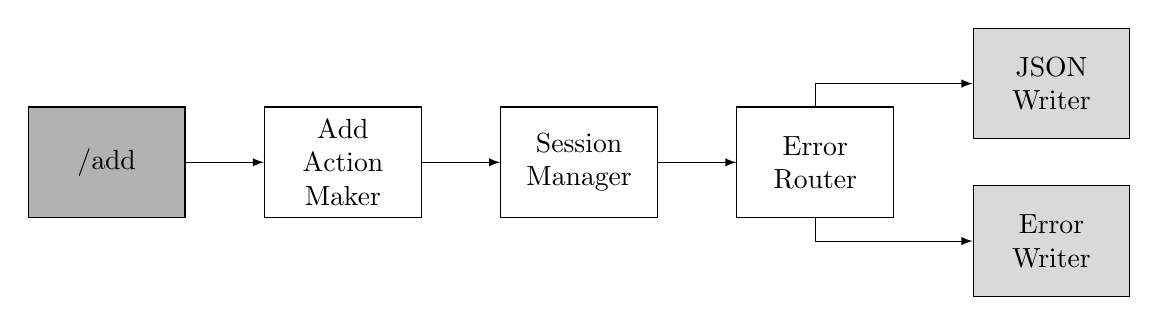
\begin{tikzpicture}[node distance = 2cm, auto]
    % Nodes
    \node [listener] (listener) {/add};
    \node [component, right of=listener, node distance=3cm] (maker) {Add Action Maker};
    \node [component, right of=maker, node distance=3cm] (manager) {Session Manager};
    \node [component, right of=manager, node distance=3cm] (splitter) {Error Router};
    \node [writer, right of=splitter, node distance=3cm, yshift=1cm] (writer) {JSON Writer};
    \node [writer, below of=writer] (ewriter) {Error Writer};
    
    % Edges
    \path [line] (listener) -- (maker);
    \path [line] (maker) -- (manager);
    \path [line] (manager) -- (splitter);
    \path [line] (splitter) |- (writer);
    \path [line] (splitter) |- (ewriter);


\end{tikzpicture}
\caption[scale=1.0]{Part of shopping server architecture.}
\label{fig:shoppingDesign}
\end{figure}

We will make each part of the network into a separate writer as in
the Proxy Server example to be able to use the \texttt{DynamicLoadBalancer}.
The code for making this writer is shown in figure \ref{fig:shoppingWriter}.
Here, we provide action maker and storage for the session manager 
as arguments of the function.

\newpage
\begin{figure}[h]
\lstinputlisting[firstline=12,lastline=35]{../examples/shoppingServer/shoppingServer.go} 
\caption[scale=1.0]{Implementation of the writer that represents the whole
pipeline for one action.}
\label{fig:shoppingWriter}
\end{figure}

The benefit of the chosen architecture that resources for the add, remove
and buy actions are allocated independently. That is, if there is lot of 
people adding items to their shopping cart, there can be more instances
of the combined writer for the add action and fewer instances for the
other two actions. The code for running the whole server is shown
in Figure \ref{fig:ShoppingCode}.
\begin{figure}[h]
\lstinputlisting[firstline=37,lastline=72]{../examples/shoppingServer/shoppingServer.go} 
\caption[scale=1.0]{Implementation of the Shopping Server.}
\label{fig:ShoppingCode}
\end{figure}

\subsection{Summary}
In this chapter I showed how to use the \texttt{mpserver} toolkit
to build a more complex web server. I also presented how resources can
be allocated independently for different tasks. The next chapter 
presents the results of performance testing of the toolkit.




%%%%%%%%%%%%%%%%%%%%%%%%%%%%%% Testing %%%%%%%%%%%%%%%%%%%%%%%%%%%%%%%%
\newpage
\section{Performance Testing}
\label{sec:test}
In order to evaluate the performance of the \texttt{mpserver} toolkit we 
need to compare it against other server architectures.
This Chapter presents the setup and results of the performance tests
that were carried on equivalent servers implemented in the \texttt{mpserver} toolkit,
in plain Go, in the \texttt{webpipes} toolkit by James Whitehead II~\cite{whitehead} 
and the Apache framework.

\subsection{Setup}
To compare the performance of the four server architectures, I 
implemented a simple file server in all of them. Their performance 
was tested on serving a 4KB static text file and a 2MB static image. 
The code for the servers that were implemented in Go is shown in Appendix~\ref{sec:testing.go}. 

To generate the load I used \texttt{httperf} tool~\cite{httperf}. To distribute 
the testing among multiple machines I used a customized version
of the \texttt{autohttperf} tool~\cite{whitehead}.
This setup is inspired by the one used in~\cite{whitehead}.
The clients timed out after 1~second to ensure the client machines would 
not have too many connections open at the same time.

The server was run on a virtual machine with quad core processor and 
8GB of RAM. The machine was running CentOS Linux release 7.3.1611 (Core)
with Linux kernel 3.10.0.
I used 2 client machines with the same specification as the server machine, 
except that they had only 4GB of RAM. The version of Go on the machines was
1.6.3 linux/amd64. The version of Apache server used was 2.4.6 (CentOS).

The servers were given all resources on the server machine. 
As the \texttt{httperf} tool is single threaded and consumes 
all resources of the processor core on which it is run, the client 
machines ran up to 3 instances of this command (the one remaining 
core was kept free to allow any other tasks to execute there and to
be able to access the machine without interfering with the tests).

\subsection{Results}
\subsubsection{Serving a small text file}
Serving a 4KB text file is an easy and quick task, so all servers were able to
respond to all requests within the given timeout window for all load levels.
The table in Figure~\ref{results} shows the average response times in milliseconds 
for each server for a given number of requests made per second. The response time is 
measured from the moment the last byte of the request was sent to the moment when the first 
byte of the response was received \cite{httperfdoc}. The table also shows a weighted 
average of the response times for each implementation.

There are results for three different versions of the servers implemented using 
the \texttt{mpserver} toolkit. These versions are as follows:
\begin{itemize}
	\item \texttt{mpserver1} - uses a simple file server as 
		  described in Section~\ref{sec:fileServer} without any load balancing

	\item \texttt{mpserver2} - uses static load balancing with 4 instances
		  of the simple file server writer

	\item \texttt{mpserver3} - uses dynamic load balancing with maximum number of 
		  workers set to 4
\end{itemize}

\begin{figure}[h]
\begin{center}
\begin{tabular}{|c|c|c|c|c|c|c|c|}
\hline
Req/s & Go & webpipes & mpserver1 & mpserver2 & mpserver3 & Apache\\
\hline
100 & 0.42 & 0.55 & 0.45 & 0.45 & 0.47 & 1.75 \\
200 & 0.40 & 0.57 & 0.53 & 0.50 & 0.62 & 1.80 \\
300 & 0.50 & 0.60 & 0.50 & 0.50 & 0.70 & 1.70 \\
400 & 0.50 & 0.60 & 0.50 & 0.43 & 0.65 & 1.68 \\
500 & 0.45 & 0.50 & 0.43 & 0.53 & 0.65 & 1.85 \\
600 & 0.45 & 0.53 & 0.47 & 0.50 & 0.80 & 1.62 \\
700 & 0.47 & 0.62 & 0.43 & 0.40 & 1.08 & 1.62 \\
800 & 0.42 & 0.55 & 0.47 & 0.47 & 1.15 & 1.70 \\
\hline
avg & 0.45 & 0.56 &	0.47 & 0.47 & 0.87 & 1.70 \\
\hline
\end{tabular}
\end{center}
\caption{Response times of different file server implementations in ms under varying loads.}
% mpserver1= simple setup
% mpserver2= static load balancer
% mpserver3= dynamic load balancer
% mpserver4= listener load balancer
\label{results}
\end{figure}

Unexpectedly the Apache server had the worst response times. This was likely due to 
overheads for authorization that were not present on the other servers. As expected,
the server implemented using plain Go gives the best results out of all the Go
implementations. 

Then second best were the implementations in the \texttt{mpserver}
toolkit, which used the simple file server and the file server with static load 
balancing. Their performance was approximately the same, because the file server is composed of 
4 parts (excluding the listener), so under a high load both implementations 
were executing 4 goroutines simultaneously. 

The \texttt{webpipes} toolkit performed slightly worse than the two best
\texttt{mpserver} implementations. As noted in Section~\ref{sec:relaedWork} this was probably
due to overheads for creating the reader-writer pairs.
The \texttt{mpserver} version using dynamic load balancing was the slowest Go implementation.
This was most likely due to the fact that the load balancer is almost always ready to perform
an operation that consumes resources, which could otherwise be used to serve requests.

\subsubsection{Serving a large image}
Serving a large image is a much slower task than serving a small text file.
Therefore the servers were not able to respond to all requests within the
given timeout window for higher loads. The table in Figure~\ref{results2} shows
the total number of connections made for each request rate and the total number
of responses received within the given timeout window for each server implementation.

\begin{figure}[h]
\begin{center}
\begin{adjustwidth}{-.5in}{-.5in} 
\begin{tabular}{|c|c|c|c|c|c|c|c|}
\hline
Req/s & \#connections & go    & webpipes & mpserver1 & mpserver2 & mpserver3 & Apache \\
\hline
100   & 16000        & 16000 & 15998    & 5859      & 10672     & 11072     & 16000 \\
200   & 32000        & 20677 & 23378    & 6017      & 10538     & 10795     & 16981 \\
300   & 48000        & 25628 & 24146    & 4693      & 9834      & 10929     & 24351 \\
400   & 64000        & 28545 & 13600    & 3670      & 10989     & 9149      & 31625 \\
500   & 80000        & 7702  & 14180    & 4391      & 10974     & 10224     & 39774 \\
600   & 96000        & 507   & 492      & 3930      & 10794     & 8773      & 20500 \\
700   & 112000       & 162   & 225      & 2223      & 9750      & 10342     & 20693 \\
800   & 128000       & 104   & 122      & 3552      & 10425     & 8905      & 20668 \\
\hline
\end{tabular}
\end{adjustwidth}
\end{center}
\caption{Total number of responses received for different file server implementations under varying loads.}
\label{results2}
\end{figure}

In this test the Apache server significantly outperformed all other implementations under 
high loads. This is to be expected as it is a mature framework with millions of users, and that has 
been optimized over the years.

The performance of the pure Go and the \texttt{webpipes} servers was very similar, because their implementations are nearly identical, with the exception
that the \texttt{webpipes} version performs additional work when writing the file back to 
the client. They were able to serve most requests for lower loads, but their performance
rapidly decreased at 600 requests per second. They were only able to serve a few hundred requests
out of the tens thousands made. 

This was probably due to the fact that each individual request is handled by a 
separate goroutine and so there was a very high number of goroutines being spawned
continuously. Hence, there might have been significant delay between the arrival of 
a request and the moment when the goroutine handling it was scheduled. 
Also every goroutine that is responding to a request blocks on a system call to 
access the requested file and gets descheduled. Again, there might be a significant
delay before this goroutine is scheduled again. Therefore most of the clients 
timeout and close the connection before the server starts sending the file.

None of the \texttt{mpserver} implementations were able to respond to all requests 
within the given timeout window, for all request rates; the maximum number 
of request they were able to handle per second was lower than 100. 
However, \texttt{mpserver2} and \texttt{mpserver3} were able to work on their maximum 
capacity for all request rates. This was due to 
the fact that goroutines handling incoming requests were almost immediately blocked
when they tried to send their \texttt{jobs} to the pipeline. Hence, the components 
in the network were able to perform their tasks, as they were almost always ready 
under the high loads. Therefore if a \texttt{job} entered the pipeline early enough,
it was most likely processed before the timeout.

The simple version without any load balancing had the worst performance as results 
can only be written to one client at a time, demonstrating the advantages of 
load balancing. The version with dynamic load balancing performed slightly worse due
to the overheads for the dynamic load balancer.

\subsection{Summary}
This Chapter presented the setup and results of the performance tests carried out.
The results for the \texttt{mpserver} toolkit are very encouraging. It is faster than
the \texttt{webpipes} toolkit and the difference between its performance and the performance
of the pure Go implementation is negligible in the case of serving a small text file.

The results for serving a large image show that the \texttt{mpserver} implementations can deal
much better with high loads when performing more expensive tasks, than the \texttt{webpipes} and
pure Go implementations. The performance of any of the Go web-servers was nowhere near as good
as the performance of the Apache server in the second test. However, as previously noted, this was to 
be expected as Apache is a mature framework.

%%%%%%%%%%%%%%%%%%%%%%%%%%%%% Conclusion %%%%%%%%%%%%%%%%%%%%%%%%%%%%%%
\newpage
\section{Conclusion}
\label{sec:conclusion}
\subsection{Summary}
I successfully developed a compositional toolkit for construction of 
web-servers in Go. I first introduced the idea behind the toolkit that 
makes the construction of web-servers very intuitive and straight forward. 

Then I presented my implementation. I started by introducing the basic types
and then went on to describe much more complicated components and component generators
that make it easy to implement complex behaviors. I demonstrated the usage of the 
toolkit on a handful of simple examples and performed a case study of building
a more complex server using the toolkit. This showed that the toolkit is
functional and simple to use. 

Finally, I also performed performance testing of the toolkit and compared
performance of file servers implemented in the toolkit to the performance
of file servers implemented using other frameworks.

\subsection{Critical analysis}
As noted above the toolkit is easy to use due the fact that response 
generation diagrams translate directly to program code. The components
in the toolkit are very general and highly configurable. The toolkit
also gives programmers control over how many resources are used for 
different tasks. 

However, the performance of servers implemented in the toolkit can be 
poor if they are not configured properly. This is because when using a simple
pipeline without any load balancing all requests must go through all parts
of the server one by one, limiting the throughput. This is an issue 
in case at least one of the components in the pipeline is performing a slow operation.
The provided tools for load balancing mitigate this problem.

The performance of the toolkit is worse than just using the standard library
on computationally cheap tasks. This is due to overheads
for the usage of channels, creating the \texttt{Job} objects
and switching between different goroutines. However, the performance
penalty is very small. Moreover the the performance for expensive 
tasks is order of magnitude better under high loads than the default implementation,
as was demonstrated by the tests carried out.

The toolkit provides a lot of functionality over the
standard library and makes implementing servers more straight forward. 
Hence, developing servers using the toolkit should be
significantly easier and therefore quicker. So, if this very small performance
penalty on cheap tasks is acceptable, then my toolkit should be the preferred 
alternative.

\subsection{Future Work}
To make the toolkit production-ready I would perform  more performance 
tests under even higher loads. I would also thoroughly test the performance of
every component in the toolkit, implement more components and improve my documentation. 

One might want to implement a version of the \texttt{Storage}
that uses an SQL database or a component that accesses a database and 
returns the requested data. As noted before, other strategies 
for load balancing can be implemented. 
They can possibly be abstracted into their own type, so that the
load manager can be parameterized based on our needs.

The library is very general and extensible. Hence, if we wanted to support 
other protocols such as webSocket we can easily implement a different 
type of \texttt{job} and associated components and writers in similar fashion.



%%%%%%%%%%%%%%%%%%%%%%%%%%%% Bibliography %%%%%%%%%%%%%%%%%%%%%%%%%%%%%
\newpage
\printbibliography[
    heading=bibintoc,
    title={References}
]

%%%%%%%%%%%%%%%%%%%%%%%%%%%%% Appendices %%%%%%%%%%%%%%%%%%%%%%%%%%%%%%
\appendix
\newpage
\begin{appendices}
\section{Example servers}

\subsection{Proxy Server Implementation}
\subsubsection{proxyServer.go}
\lstinputlisting{../examples/proxyServer/proxyServer.go}

\newpage
\subsection{Shopping Server Implementation}
\subsubsection{actions.go}
\lstinputlisting{../examples/shoppingServer/actions.go}
\subsubsection{shoppingCart.go}
\lstinputlisting{../examples/shoppingServer/shoppingCart.go}
\subsubsection{actionMakers.go}
\lstinputlisting{../examples/shoppingServer/actionMakers.go}
\newpage
\subsubsection{shoppingServer.go}
\lstinputlisting{../examples/shoppingServer/shoppingServer.go}
\end{appendices}

\end{document}




